\mychapter{Demonstração de uso do Software}{cap:demonstracao}

Nesta sessão, demonstraremos como utilizar a interface do Software desenvolvido para realizar a análise da caracterização do ruído colorido\footnote{\url{https://www.mathworks.com/matlabcentral/fileexchange/35381-noisefk-m}} de espectro de potência $f^{-3/2}$.

\section{Upload de dados} 

Primeiramente, iremos fazer upload do arquivo $.csv$ que contém os dados que serão utilizados. Para isso iremos clicar no botão \mybox{BROWSE} e selecionar o arquivo desejado (Figura~\ref{fig:Upload}).

\begin{figure}[H]
	\centering
	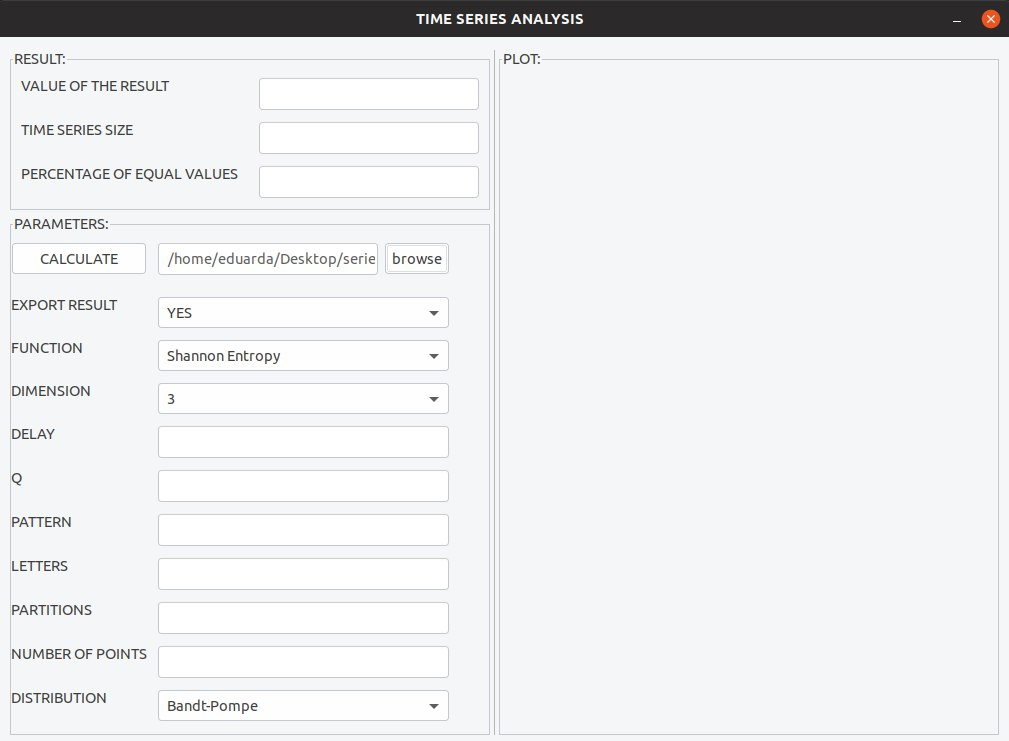
\includegraphics[width=0.85\columnwidth]{capitulos/imagens/Upload} 
    \caption{Upload do arquivo}
    \label{fig:Upload}
\end{figure}

\section{Visualização da série temporal}

O próximo passo será visualizar como se comporta a série temporal ao longo do tempo. Para isso, iremos selecionar dentro das possibilidades da variável \mybox{FUNCTION} a funcionalidade \mybox{Time Series Plane}.

Como podemos verificar, algumas informações básicas sobre os dados também são fornecidas, como o tamanho da série e o percentual de valores repetidos (Figura~\ref{fig:TimeSerie}).

O software disponibiliza a opção de exportar os resultados obtidos em cada iteração com o usuário, para isso é necessário apenas habilitar a opção na variável \mybox{EXPORT RESULT}. 
Essa funcionalidade promove a reprodutibilidade dos estudos.
Todos os  arquivos resultantes são armazenados no mesmo diretório que o sistema se encontra.


\begin{figure}[H]
	\centering
	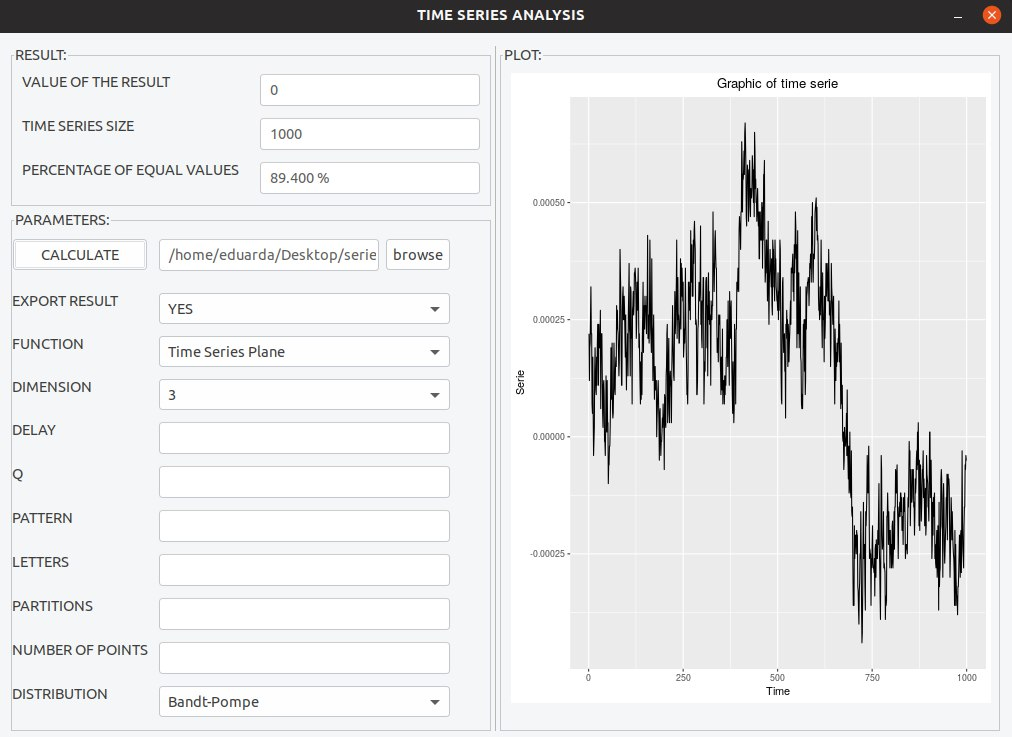
\includegraphics[width=0.85\columnwidth]{capitulos/imagens/timeSeriesPlot} 
    \caption{Gráfico do comportamento da Série Temporal}
    \label{fig:TimeSerie}
\end{figure}

\section{Histograma da distribuição de Bandt-Pompe} 

Assim como propõe a metodologia da simbolização, iremos agora visualizar como se comporta a distribuição dos padrões de Bandt-Pompe. Neste exemplo, aplicaremos valores de dimensão $D = 3$ e delay $\tau = 1$. Para isso, selecionaremos a funcionalidade \mybox{Histogram} e configuraremos a variável \mybox{DELAY} para o valor desejado (Figura~\ref{fig:bandtPompe}).

\begin{figure}[H]
	\centering
	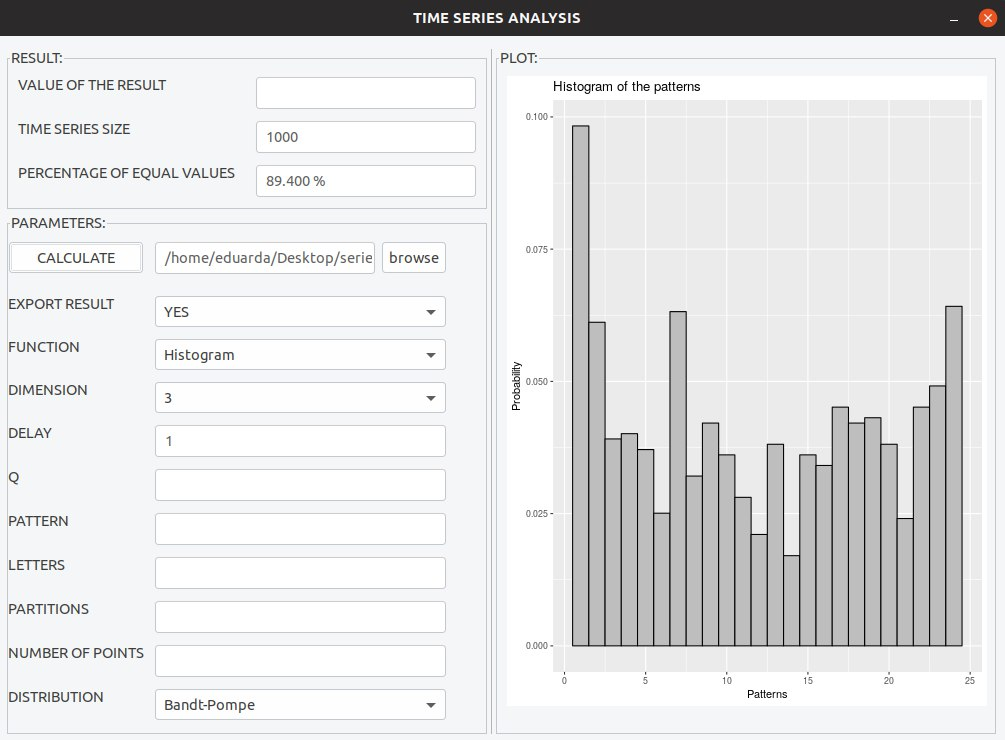
\includegraphics[width=0.85\columnwidth]{capitulos/imagens/Histogram} 
    \caption{Histograma da distribuição da probabilidade de Bandt-Pompe}
    \label{fig:bandtPompe}
\end{figure}

\section{Cálculo da Entropia de Shannon}

Para adquirir isoladamente o valor da Entropia de Permutação Normalizada de Shannon, devemos agora apenas selecionar a opção \mybox{Shannon Entropy} e pressionar o botão \mybox{CALCULATE} (Figura~\ref{fig:shannon}).

\begin{figure}[!hbt]
	\centering
	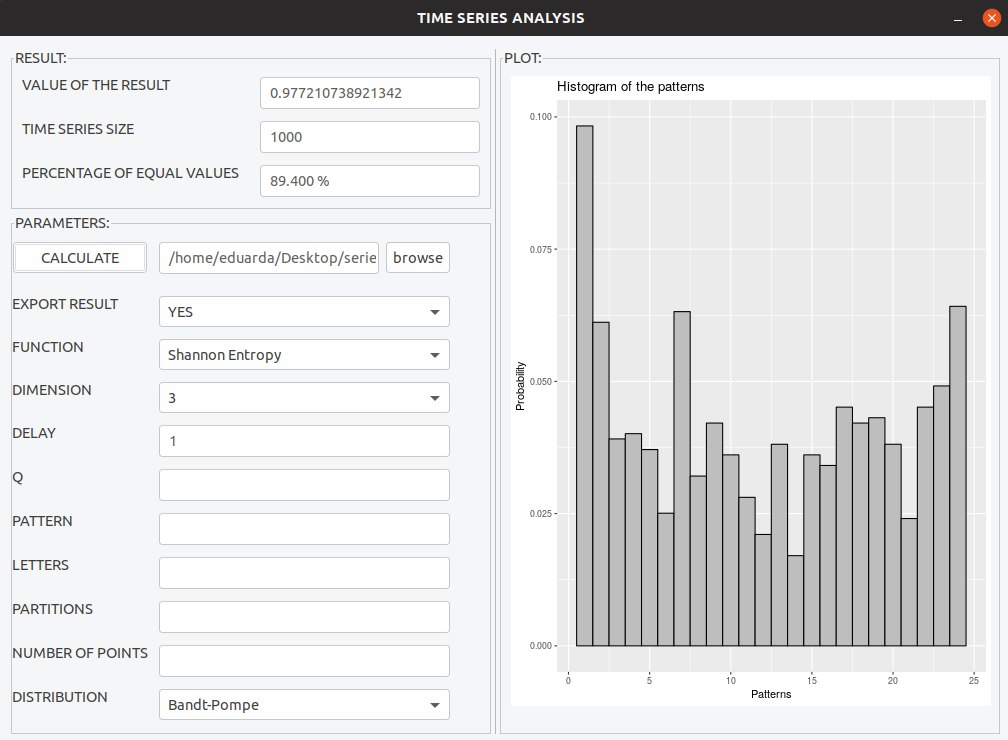
\includegraphics[width=0.85\columnwidth]{capitulos/imagens/Shannon} 
    \caption{Resultado obtido da Entropia de Shannon}
    \label{fig:shannon}
\end{figure}

\section{Cálculo da Complexidade Estatística}

De modo semelhante a Entropia, para possui o valor da Complexidade Estatística, devemos selecionar a opção \mybox{Statistical Complexity} e pressionar o botão \mybox{CALCULATE} (Figura~\ref{fig:complexity}).

\begin{figure}[!hbt]
	\centering
	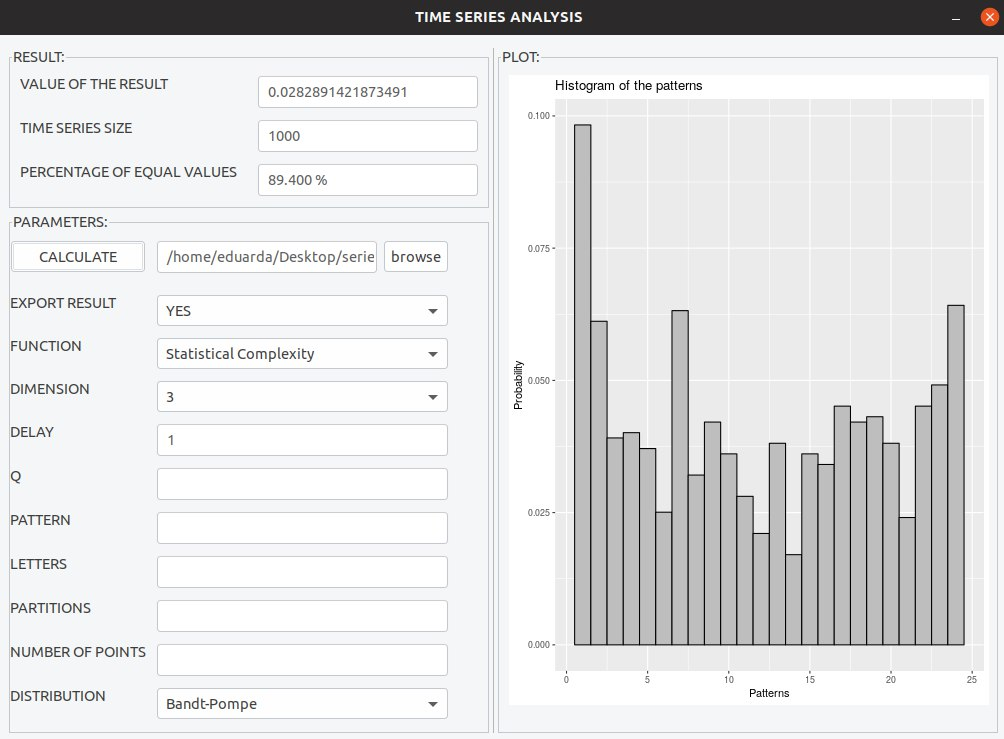
\includegraphics[width=0.85\columnwidth]{capitulos/imagens/complexity} 
    \caption{Resultado obtido da Complexidade Estatística}
    \label{fig:complexity}
\end{figure}

\section{Plano Complexidade-Entropia}

Por fim, uma vez que os valores referentes a dimensão $D$ e o delay $\tau$ já se encontram configurados, para gerar o Plano Complexidade-Entropia devemos apenas selecionar a opção \mybox{HC Plane} e informar em quantas partições queremos analisar a série, caso o valor informado seja superior a 1, a série irá ser dividida em subconjuntos e exibido os pontos correspondentes a cada um destes (Figura~\ref{fig:hCPlane}).

Como podemos observar, o comportamento descrito no plano corresponde ao valor já esperado na literatura~\citep{phdthesis}, o ruído $f^{-3/2}$ possui um alto valor de Entropia, ou seja alta desordem na estrutura da dinâmica dos seus dados e um baixo valor de Complexidade.

\begin{figure}[!hbt]
	\centering
	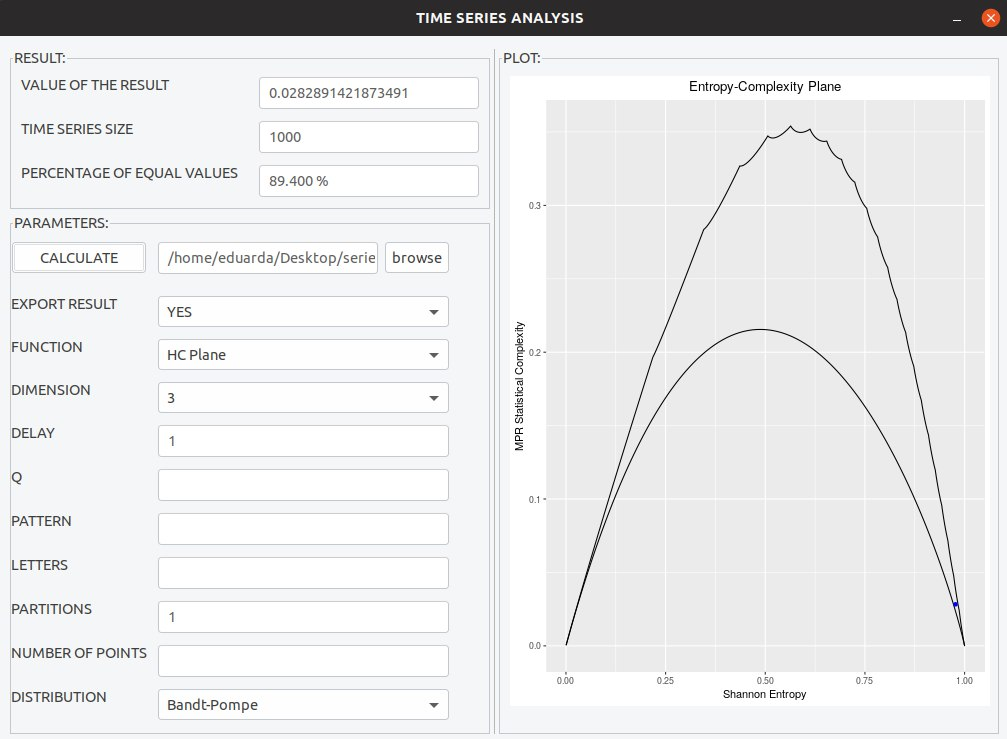
\includegraphics[width=0.85\columnwidth]{capitulos/imagens/hCPlane} 
    \caption{Caracterização do ruído $f^{-3/2}$ no Plano Complexidade-Entropia}
    \label{fig:hCPlane}
\end{figure}